% gr-Moser.tex -- the Moser spindle : 7 vertices, 11 edges, all of
% length 1 ; it needs 4 colours (Hadwiger-Nelson problem : at least 4
% colours for the plane). Engine : pdfLaTeX or LuaLaTeX
\documentclass[border=3mm, convert=false]{standalone}
\usepackage{tkz-berge}
\begin{document}
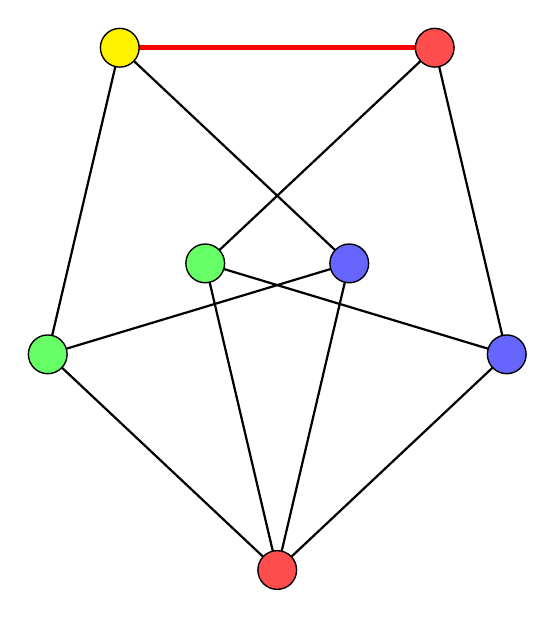
\begin{tikzpicture}[scale=4]
  \GraphInit[vstyle=Normal]
  \SetVertexNoLabel
  \tikzset{VertexStyle/.append style = {minimum size = 14pt}}
  % theta : the two spindles turn so that their tips are at distance 1
  \pgfmathsetmacro\t{2*asin(1/(2*sqrt(3)))}
  \pgfmathsetmacro\u{90-\t/2}
  \pgfmathsetmacro\w{90+\t/2}
  \tikzset{c1/.style={fill=red!70},c2/.style={fill=blue!60},
           c3/.style={fill=green!60},c4/.style={fill=yellow}}
  \coordinate (A) at (0,0);
  \coordinate (B) at (\u-30:1);  \coordinate (C) at (\u+30:1);
  \coordinate (D) at (\u:{sqrt(3)});
  \coordinate (E) at (\w-30:1);  \coordinate (F) at (\w+30:1);
  \coordinate (G) at (\w:{sqrt(3)});
  \Edges(A,B,D,C,A) \Edge(B)(C)
  \Edges(A,E,G,F,A) \Edge(E)(F)
  \Edge[local,color=red,lw=2pt](D)(G)
  \foreach \v/\c in {A/c1,B/c2,C/c3,D/c1,E/c2,F/c3,G/c4}
    {\node[VertexStyle,\c] at (\v) {};}
\end{tikzpicture}
\end{document}
